%!TEX root = ../../report.tex

\subsubsection{Shape Grammars} % (fold)
\label{ssub:shape_grammars}


Shape Grammars can be considered grammars for design. Instead of having symbols or letters as components of the alphabet, it has shapes that can be in 2D or 3D, and has production rules that are composed by these shapes, that specify the evolution of the system. With this process, similar to the L-Systems explained before, the shape starts from a seed, i.e. a usually simple shape and can evolve to one big and/or complex shape.

The process is performed in two steps, the recognition of a shape and the replacement according to the rules previously defined. 

Figure~\ref{fig:SGrammars} exemplifies one shape grammar with one rule, and the evolution of the application of this rule to the shapes iteratively. In this image, it is shown that from very simple initial shape, a complex from can be generated after a few iterations.

\begin{figure}
        \centering
		%\begin{subfigure}[b]{0.55\textwidth}
			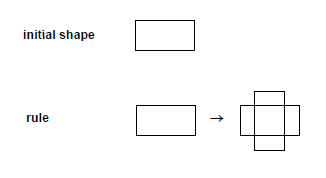
\includegraphics[width=0.45\textwidth]{img/Theory/Shape_Grammars/Grammar.png}
			%\caption{a)}
			%\label{fig:SGGrammar}
		%\end{subfigure}
        
         %add desired spacing between images, e. g. ~, \quad, \qquad, \hfill etc.
          %(or a blank line to force the subfigure onto a new line)
		%\begin{subfigure}[b]{0.55\textwidth}
			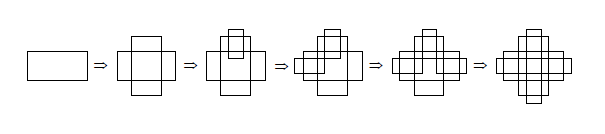
\includegraphics[width=0.45\textwidth]{img/Theory/Shape_Grammars/Recursion.png}
			%\caption{b)}
			%\label{fig:SGRecursion}
		%\end{subfigure}
        \caption{a) Grammar Tiles b) Recursion steps}
        \label{fig:SGrammars}
\end{figure}

In the CityEngine \cite{Muller2006} system, this is applied to the generation of buildings using 3D blocks for the main form, and 2D shapes to design the facades.

% \begin{figure}[htbp]
% 	\centering
% 	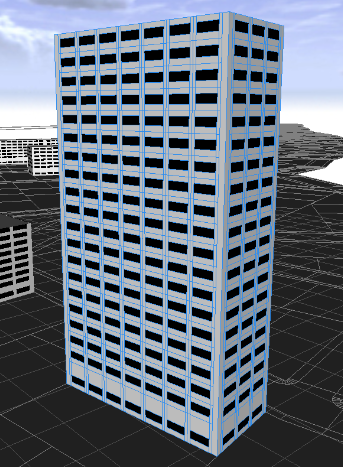
\includegraphics[width=0.55\textwidth]{img/Theory/Shape_Grammars/Edificio.png}
% 	\caption{Simple Building}
% 	\label{fig:SGBuilding}
% \end{figure}

Figure~\ref{fig:SGBuilding} shows a simple building that I modelled using CityEngine and its CGA Shape Grammar (Section~\ref{sub:cityengine}). But CGA is powerful enough to model much more complex buildings like the one in Figure~\ref{fig:CEBuilding}.


% \begin{figure}[htbp]
% 	\centering
% 	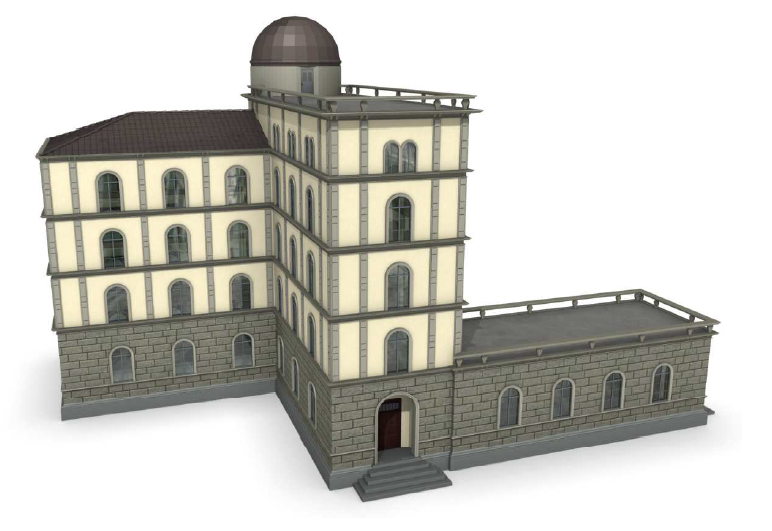
\includegraphics[width=0.55\textwidth]{img/Theory/Shape_Grammars/Capturar.png}
% 	\caption{Complex Building \cite{Muller2006}}
% 	\label{fig:CEBuilding}
% \end{figure}

\begin{figure}
\centering
\begin{minipage}{.48\textwidth}
  \centering
  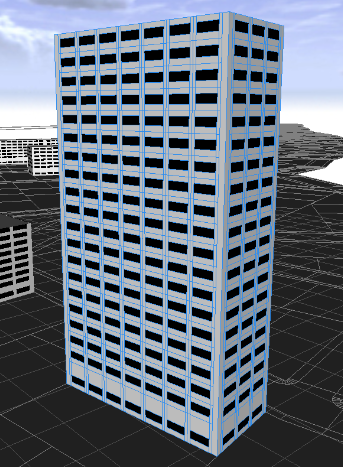
\includegraphics[width=.5\linewidth]{img/Theory/Shape_Grammars/Edificio.png}
  \captionof{figure}{Simple Building}
  \label{fig:SGBuilding}
\end{minipage}
~~
\begin{minipage}{.48\textwidth}
  \centering
  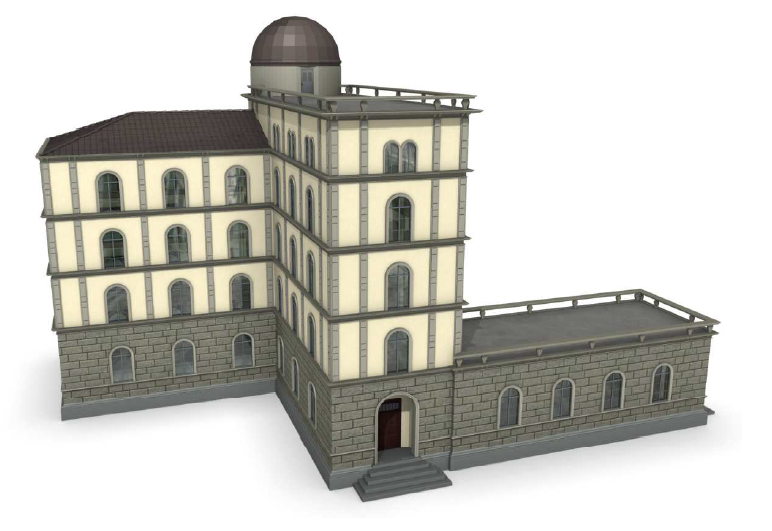
\includegraphics[width=0.8\linewidth]{img/Theory/Shape_Grammars/Capturar.png}
  \captionof{figure}{Complex Building \cite{Muller2006}}
  \label{fig:CEBuilding}
\end{minipage}
\end{figure}

% subsubsection shape_grammars (end)